\subsection{Representation: RTE as AST}


{  %\setbeamercolor{background canvas}{bg=sectioncolor}
\begin{frame}{\Challenge{1} RTE Representation}

  How to represent an RTE in Clojure, Scala, Python, etc...?


  \medskip
  
  %% \begin{itemize}
  %% \item Surface syntax: declarative, expressive, composable
  %% \item Programmatic interface: reflective, algebraic manipulation
  %% \end{itemize}
\end{frame}
}

\newsavebox\exnoteboxscala
\begin{lrbox}{\exnoteboxscala}
  \begin{minipage}{6.5cm}
    %% dont re-indent this file
\begin{lstlisting}[style=reclojureScala]
val I:Rte = Atomic(classOf[Int])
val F:Rte = Atomic(classOf[Float])
val odd:Rte = Satisfies(oddp, "odd")

val re:Rte = (I ++ (F | odd).+ ).*
\end{lstlisting}

  \end{minipage}
\end{lrbox}

\newsavebox\exnoteboxclojure
\begin{lrbox}{\exnoteboxclojure}
  \begin{minipage}{6.5cm}
    %% dont re-indent this file
\begin{lstlisting}[style=reclojureClojure]
(:* (:cat Integer 
          (:+ (:or Float
                   (:satisifes oddp)))))
\end{lstlisting}

  \end{minipage}
\end{lrbox}

\newsavebox\exnoteboxpython
\begin{lrbox}{\exnoteboxpython}
  \begin{minipage}{6.5cm}
    %% dont re-indent this file
\begin{lstlisting}[style=reclojurePython]
rt = Star( Cat( Atomic(int),
                Plus( Or( Atomic(float)
                          Satisfies(oddp, "odd")))))
\end{lstlisting}

  \end{minipage}
\end{lrbox}


\begin{frame}[t]{RTEs}{PL Declarative, Composable Syntax}
  \begin{columns}
    \begin{column}{0.55\textwidth}
  \begin{itemize}
  \item Mathematical notation:\\
  \quad\textcolor{greeny}{$(Int \cdot (Float \cup odd)^+)^*$}

  \item Leaf nodes interface to native type system

  \item \only<3>{ Scala notation:\\
    \usebox\exnoteboxscala}%
  \only<2>{ Python notation:\\
    \usebox\exnoteboxpython}%
  \only<1>{ Clojure notation:\\
    \usebox\exnoteboxclojure}%
  \end{itemize}
    \end{column}%
    \begin{column}{0.45\textwidth}
      \scalebox{0.7}{% Modeled after the following
% A simple Tree
% Author: Stefan Kottwitz
% https://www.packtpub.com/hardware-and-creative/latex-cookbook
\documentclass[border=10pt]{standalone}
\usepackage{tikz}
\begin{document}
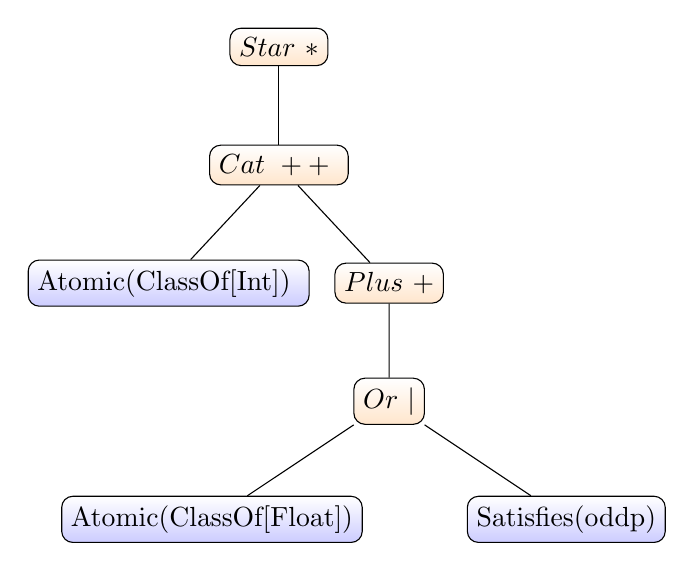
\begin{tikzpicture}[sibling distance=10em,
  every node/.style = {shape=rectangle, rounded corners,
    draw, align=center,
    top color=white, bottom color=orange!20}]]
    \tikzstyle{level 2}=[sibling distance=28mm]
    \tikzstyle{level 4}=[sibling distance=45mm]
  \node {$Star~*$}
  child { node { $Cat~++$ } 
    child { node [bottom color=blue!20] {\text{Atomic(ClassOf[Int])} }}
    child { node {$Plus~+$} 
      child { node {$Or~|$}
        child { node [bottom color=blue!20] {\text{Atomic(ClassOf[Float])}} }
        child { node [bottom color=blue!20] {\text{Satisfies(oddp)}} } } } } ;
\end{tikzpicture}
\end{document}
}
    \end{column}%
  \end{columns}%
\end{frame}


\newsavebox\exampleAbox
\begin{lrbox}{\exampleAbox}
  \begin{minipage}{12cm}
    %% dont re-indent this file
\begin{lstlisting}[style=reclojureScala]
val data = Seq("C", 100, 200, 300,
                 "M", 10.0, 20.0,
                 "M",
                 "C", 1, 2, 3,
                 "C", 1, 3, 7, 8)
\end{lstlisting}

  \end{minipage}
\end{lrbox}



\newsavebox\exampleAbbox
\begin{lrbox}{\exampleAbbox}
  \begin{minipage}{12cm}
    %% dont re-indent this file
\begin{lstlisting}[style=reclojureScala]
val data = Seq("C", 100, 200, 300, // count
                 "M", 10.0, 20.0, // measurement
                 "M",
                 "C", 1, 2, 3,
                 "C", 1, 3, 7, 8)

val F:Rte = Atomic(classOf[Double]) | Atomic(classOf[Float])
val I:Rte = Atomic(classOf[Int])
val keyM:Rte = Eql("M")
val keyC:Rte = Eql("C")

val re:Rte = ((keyC ++ I.*) | (keyM ++ F.*)).*

re.contains(data) // returns true
\end{lstlisting}

  \end{minipage}
\end{lrbox}



\newsavebox\exampleAcbox
\begin{lrbox}{\exampleAcbox}
  \begin{minipage}{12cm}
    %% dont re-indent this file
\begin{lstlisting}[style=reclojureScala]
val bad   = Seq("C", 100, 200, 300,
                 "M", 10.0, 20.0,
                 "M",
                 "C", 1, ~~2.0~~, 3, // VIOLATES PATTERN
                 "C", 1, 3, 7, 8)

val F:Rte = Atomic(classOf[Double]) | Atomic(classOf[Float])
val I:Rte = Atomic(classOf[Int])
val keyM:Rte = Eql("M")
val keyC:Rte = Eql("C")

val re:Rte = ((keyC ++ I.*) | (keyM ++ F.*)).*

re.contains(~~bad~~) // returns false
\end{lstlisting}

  \end{minipage}
\end{lrbox}



\newsavebox\exampleAdbox
\begin{lrbox}{\exampleAdbox}
  \begin{minipage}{12cm}
    %% dont re-indent this file
\begin{lstlisting}[style=reclojureScala]
val F = Atomic(classOf[Double]) | Atomic(classOf[Float])
val I = Atomic(classOf[Int])
val keyM = Eql("M")
val keyC = Eql("C")

val re:Rte = ((keyC ++ I.*) | (keyM ++ F.*)).*
\end{lstlisting}

  \end{minipage}
\end{lrbox}




\newsavebox\extendedbox
\begin{lrbox}{\extendedbox}
  \begin{minipage}{12cm}
  %% dont re-indent this file
\begin{lstlisting}[style=reclojureScala]
// binary infix operators
r1 & r2 == And(r1,r2)
r1 | r2 == Or(r1,r2)
r1 ++ r2 == Cat(r1,r2)
!re == Not(re)

re.* == Star(re) // zero or more

re.+ == re ++ re.* // one or more

re.? == EmptySeq | re // zero or one
\end{lstlisting}

  \end{minipage}
\end{lrbox}
